%
% $RCSfile: spread_functionality.tex,v $
%
% Copyright (C) 2002-2008. Christian Heller.
%
% Permission is granted to copy, distribute and/or modify this document
% under the terms of the GNU Free Documentation License, Version 1.1 or
% any later version published by the Free Software Foundation; with no
% Invariant Sections, with no Front-Cover Texts and with no Back-Cover
% Texts. A copy of the license is included in the section entitled
% "GNU Free Documentation License".
%
% http://www.cybop.net
% - Cybernetics Oriented Programming -
%
% http://www.resmedicinae.org
% - Information in Medicine -
%
% Version: $Revision: 1.1 $ $Date: 2008-08-19 20:41:09 $ $Author: christian $
% Authors: Christian Heller <christian.heller@tuxtax.de>
%

\subsection{Spread Functionality}
\label{spread_functionality_heading}
\index{Spread Functionality}
\index{Redundant Code}
\index{Overlapping Code through Concerns}
\index{Spread Functionality through Concerns}
\index{Layer Supertype Pattern}
\index{Lifecycle Method}
\index{Concern-less Development}
\index{Class Hierarchy}
\index{Ontology}

\begin{figure}[ht]
    \begin{center}
        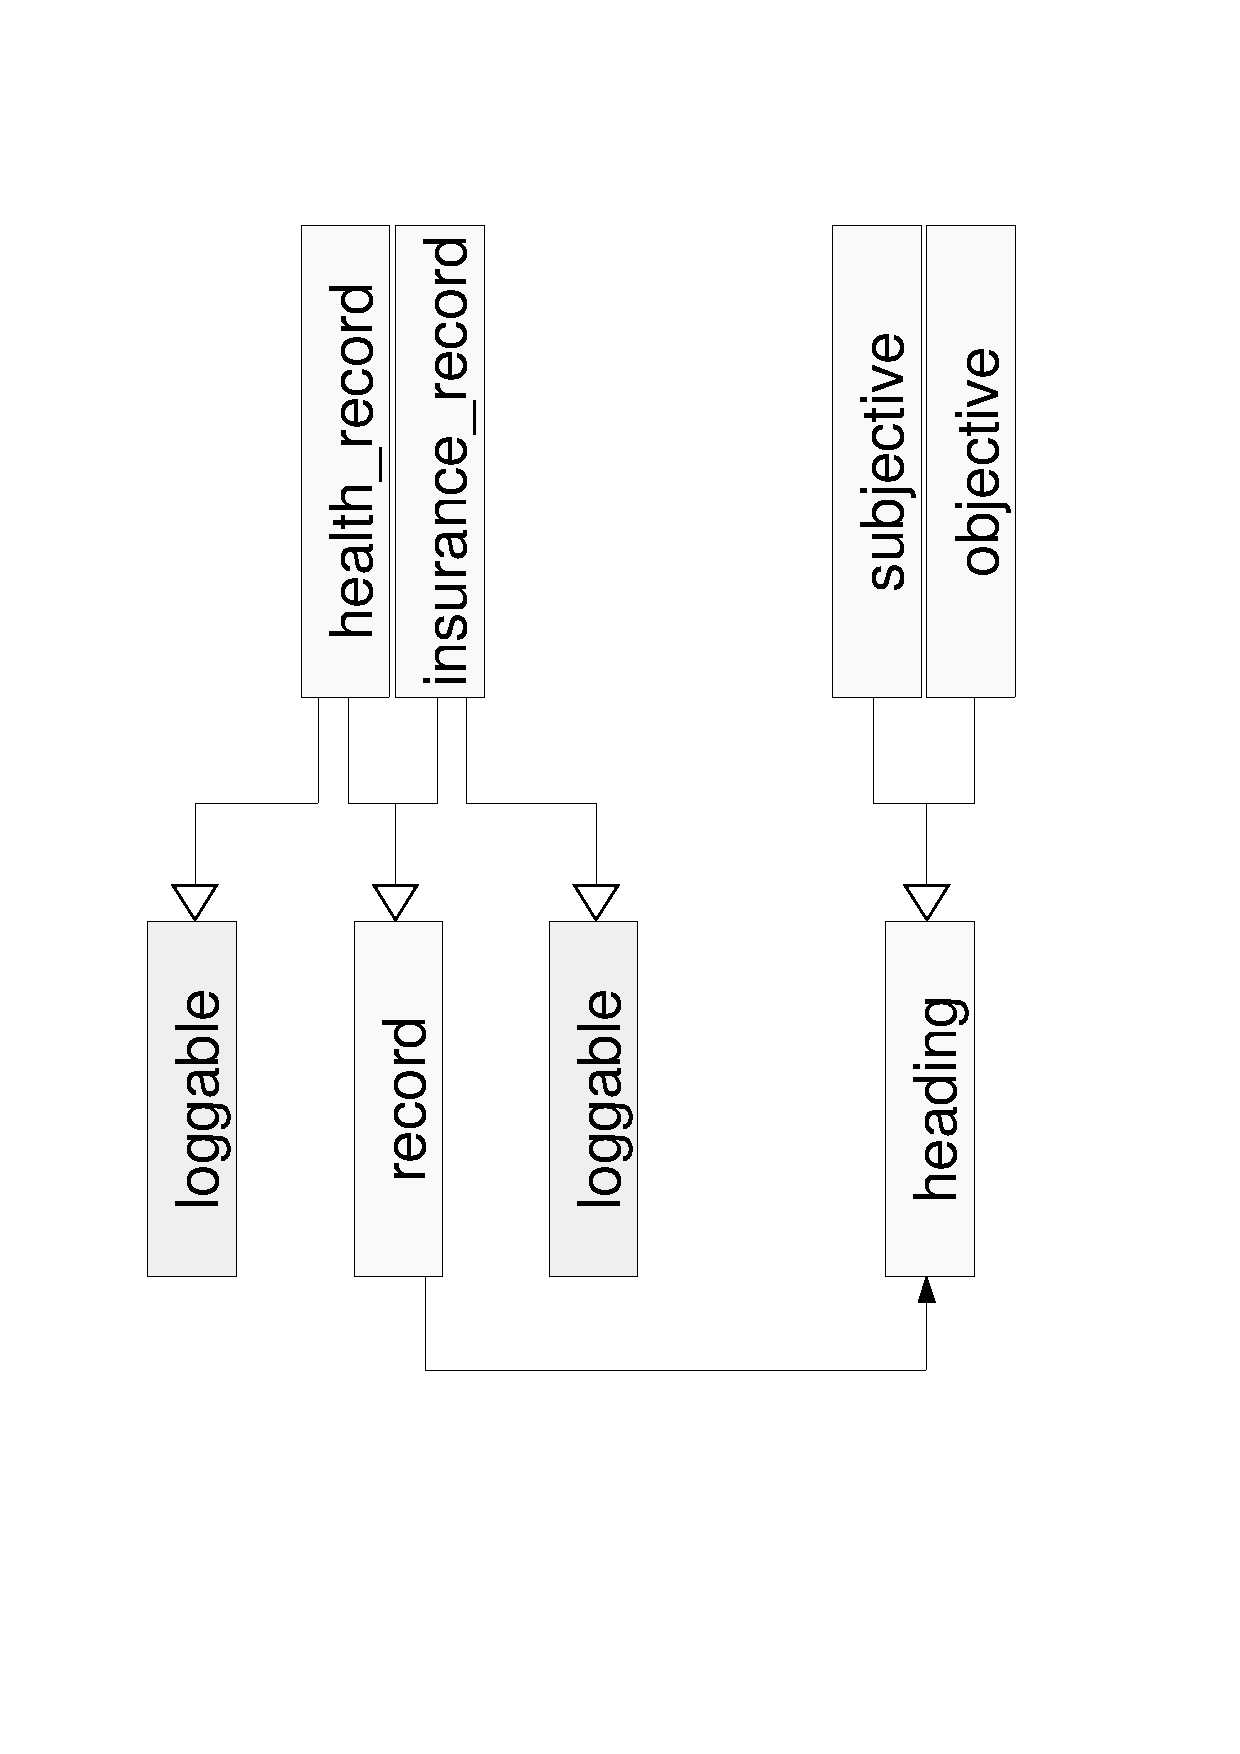
\includegraphics[scale=0.3,angle=-90]{graphic/redundant.pdf}
        \caption{Redundant Code through Usage of Concerns}
        \label{redundant_figure}
    \end{center}
\end{figure}

Separating concerns does not avoid \emph{Redundant Code}. If two independent
components want to target the same concern what they expose by implementing the
corresponding interface, they will both have to implement the required methods
redundantly. This may not be a problem with just two records as in the example
of figure \ref{redundant_figure}, but will become an issue as soon as other
objects are to be programmed as component as well.

Another unwanted effect when using concern interfaces is the \emph{Overlapping}
of concerns (figure \ref{overlapping_figure}). It may happen that a superclass
implements a number of lifecycle methods and their corresponding interfaces
without knowing if its subclasses eventually implement exactly one of these,
too. In such a case, redundant code would appear and the principle of efficient
programming would be injured once more.

\begin{figure}[ht]
    \begin{center}
        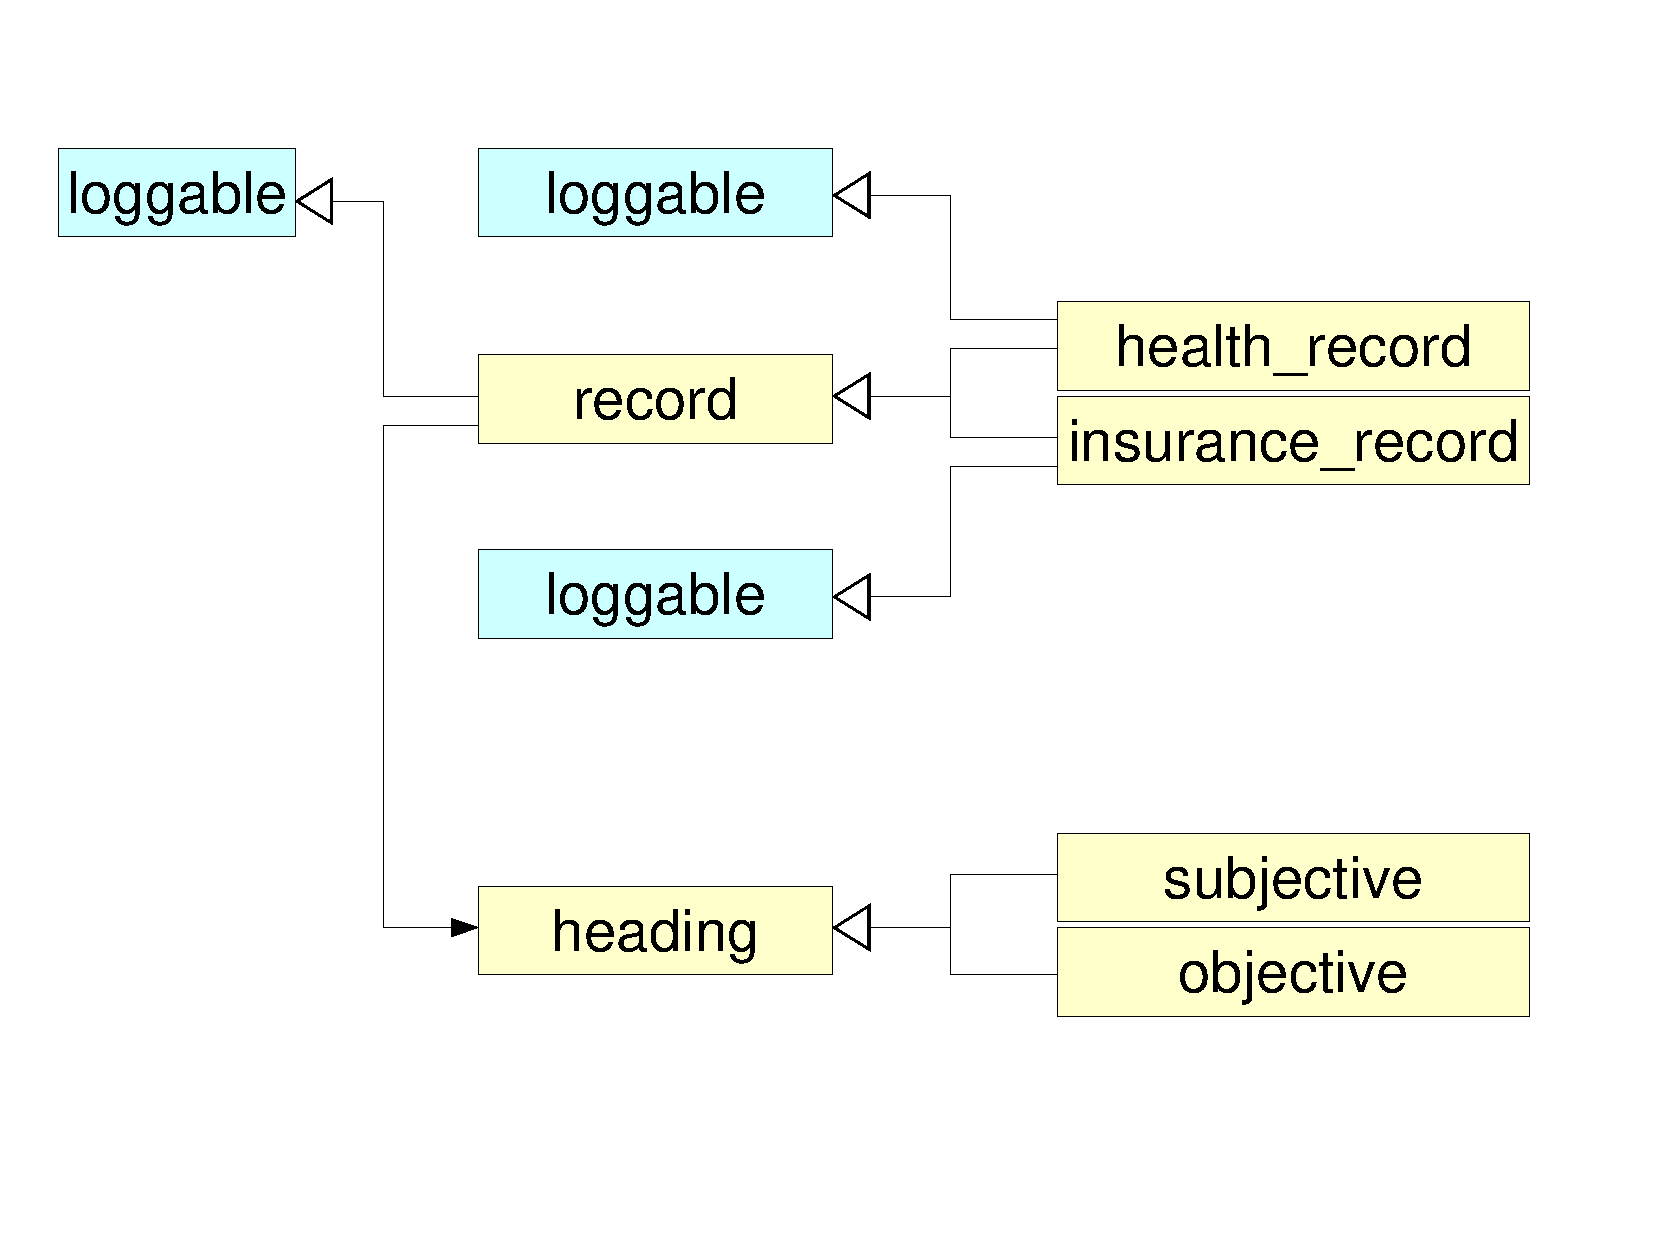
\includegraphics[scale=0.3,angle=-90]{graphic/overlapping.pdf}
        \caption{Overlapping Code through Usage of Concerns}
        \label{overlapping_figure}
    \end{center}
\end{figure}

A piece of source code holding a reference to a component instance in form of
a concern interface can \emph{only} call the methods of \emph{that} concern.
Mostly, however, other methods have to be called as well. In this case, a
\emph{Downcast} from the concern interface to the component class implementing
the interface becomes necessary. Yet to be able to downcast, the class (type)
to downcast to needs to be known anyway. In the end, the usability of concern
interfaces turns out to be limited, sometimes even useless, since they only
allow a few methods to be called and information about the real class is not
available.

\begin{figure}[ht]
    \begin{center}
        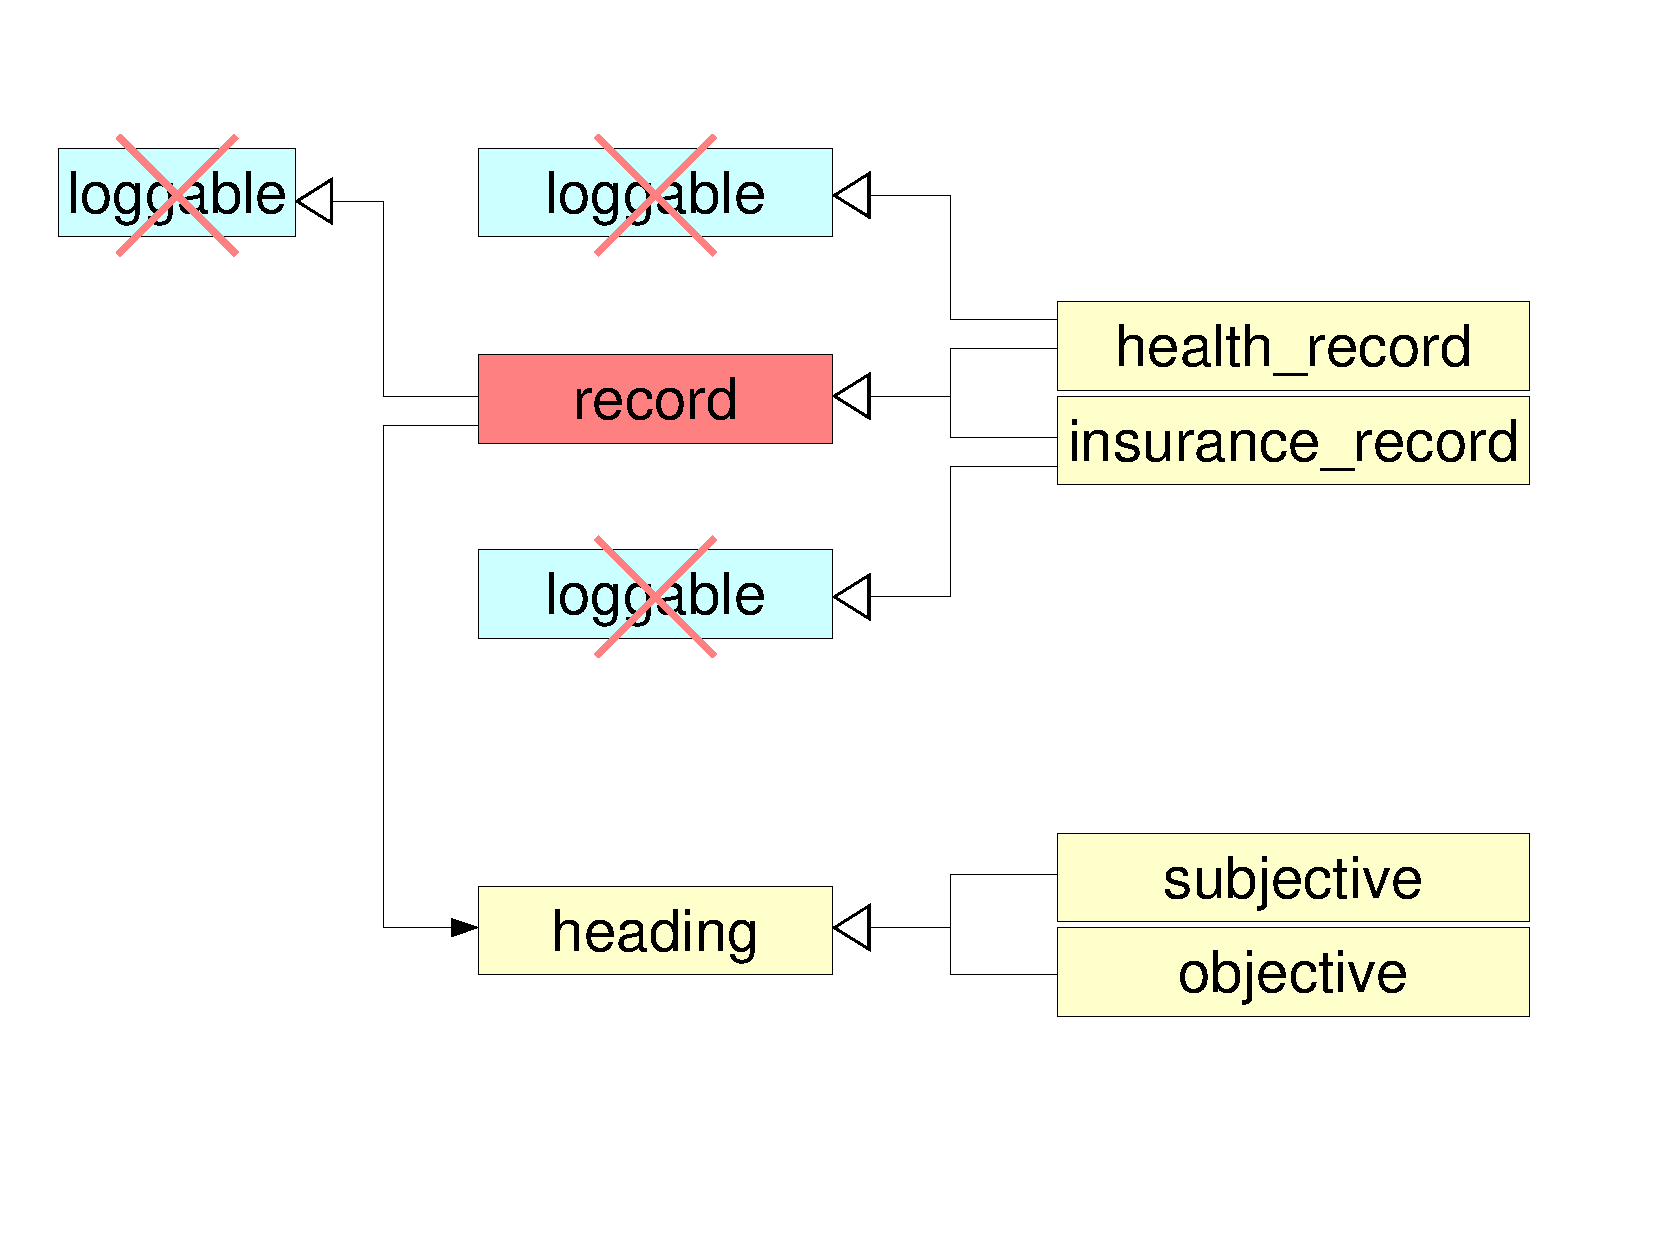
\includegraphics[scale=0.3,angle=-90]{graphic/spreadbunch.pdf}
        \caption{Concerns Spread Functionality, an Ontology Bunches it}
        \label{spreadbunch_figure}
    \end{center}
\end{figure}

From the viewpoint of reuse, it seems far better to inherit all components from
one common super-class, as suggested by the \emph{Layer Supertype} pattern
(section \ref{layer_supertype_heading}). This class would implement necessary
lifecycle methods just once, being available for all inheriting classes. For the
used example this would mean to eliminate all \emph{Loggable} concern interfaces
(figure \ref{spreadbunch_figure}) and put the logging functionality into the
\emph{Record} super class.

Finally, the only way out of the misery of redundant code caused by concern
interfaces seems to be \emph{Concern-less} software development using
\emph{pure} class hierarchies. And in fact, this is what \emph{Ontologies}
(section \ref{ontology_heading}) are proposing. Section
\ref{separation_of_concerns_heading} mentioned that interfaces help
\emph{pooling} common methods; but in the big system picture, they actually
\emph{spread} them. While concerns represented by interfaces \emph{spread}
functionality, away from the classes that were actually made to \emph{keep} it,
an ontology \emph{bunches} functionality. Chapter \ref{knowledge_schema_heading}
will show some ontology examples and introduce a knowledge schema for their
hierarchical representation, including necessary meta information.
